% =====================================================================
% SCP-LPA: Linguistic-Prior Supervised Contrastive Prototypical
% Networks for Long-Tail Few-Shot Arabic Dialect Identification
% Anonymous ACL/NAACL submission
% =====================================================================

\documentclass[11pt]{article}

\usepackage[review]{acl}
\usepackage{amsmath}
\usepackage{amsthm}
\usepackage{times}
\usepackage{latexsym}
\usepackage[T1]{fontenc}
\usepackage[utf8]{inputenc}
\usepackage{microtype}
\usepackage{makecell}
\usepackage{inconsolata}
\usepackage{graphicx}
\usepackage{amssymb}
\usepackage{booktabs}
\usepackage{multirow}
\usepackage{xcolor}
\usepackage{subcaption}
\usepackage{url}
\usepackage{float}
\usepackage{placeins}
\usepackage{enumitem}

\hypersetup{colorlinks=true, linkcolor=black, citecolor=black, urlcolor=blue}

\graphicspath{{./figs/}}

\setlength{\columnsep}{0.6cm}
\setlength{\columnseprule}{0pt}
\setlength{\textfloatsep}{6pt plus 1pt minus 1pt}
\setlength{\floatsep}{6pt plus 1pt minus 1pt}
\setlength{\intextsep}{6pt plus 1pt minus 1pt}
\setlength{\abovecaptionskip}{2pt}
\setlength{\belowcaptionskip}{2pt}
\linespread{0.95}

\newcommand{\bench}{ADIBench}

\title{SCP-LPA: Linguistic-Prior Supervised Contrastive Prototypical
Networks for Long-Tail Few-Shot Arabic Dialect Identification}

\author{Anonymous \\
  \texttt{\{anonymous\}@anonymous.edu} \\
  Anonymous Institution}

\date{}

\begin{document}
\maketitle

\begin{abstract}
Long-tail Arabic dialect identification (ADI) is challenging
because standard fine-tuning collapses to majority-class
prediction even at moderate imbalance ratios (5.8:1). We
introduce \textbf{LPA} (\textbf{L}inguistic-\textbf{P}rior
\textbf{A}ggregation), a test-time-only modification of
Prototypical Networks that replaces each class prototype with
a weighted average of itself and its \emph{linguistically
related} siblings, where the weights come from a
dialectological distance matrix \citep{Versteegh2006,
Habash2010}. We additionally study \textbf{SCP} (\textbf{S}upervised
\textbf{C}ontrastive \textbf{P}re-training), which replaces the
cross-entropy encoder objective with a contrastive one. We
evaluate both on \bench{}, a new multi-granularity benchmark
that unifies three Arabic dialect corpora (NADI 2024 18-way,
NADI 2024 5-way coarse, amgadhasan 5-city) and re-implements
seven published few-shot baselines. Our key findings are
threefold. \textbf{(1)} In the few-shot ($5$-way $k$-shot) regime,
all fine-tuning methods (FineTune, Focal, CB, MAML) collapse to
chance (0.20) on every dataset and seed,
extending the failure mode first reported at a 7000:1 ratio
\citep{DACD2024} to the moderate 5.8:1 regime. A class-balanced control shows that the collapse is driven by the
support-set size per class, not class imbalance.
 A support-size sweep confirms this is not a small-$k$ artefact:
 with $k$ swept over $\{1,3,5,10,20\}$, FineTune remains at chance
 ($0.199$--$0.204$) at every support size while ProtoNet improves
 monotonically ($0.401{\rightarrow}0.611$; Appendix Figure~A.1).
 Even twenty labelled examples per class do not stabilise the
 fine-tuned decision boundary.

 Macro-F1, which penalises minority-class errors far more harshly,
 leaves the ordering intact while sharpening the collapse:
 FineTune falls to $0.07$--$0.13$ (vs.\ its already-low accuracy
 of ${\approx}0.20$), whereas the metric-learning methods stay
 within $0.02$ of their accuracy (Appendix Table~A.5). \textbf{(2)}
Both LPA and SCP individually recover $\sim$3 percentage points
over ProtoNet on all six (dataset, shot) cells. \textbf{(3)}
The two mechanisms do \emph{not} stack: combining them yields
no marginal gain, because they treat the same underlying
failure (minority-class feature collapse). We argue that LPA is
therefore the more valuable contribution---a lightweight,
domain-specific prior that matches the performance of full
re-training at a fraction of the cost.
\end{abstract}

\section{Introduction}
Arabic dialect identification (ADI) is foundational for Arabic
NLP \citep{Al-Badrashiny2024,Bouamor2019}. The NADI 2024 shared
task covers 18 country-level dialects, with sample counts
ranging from 9.5K (Yemen) to 55K (Egypt)---a 5.8$\times$
long-tail ratio \citep{Al-Badrashiny2024}. Most dialects are
severely under-represented, and standard supervised training
degenerates to majority-class prediction at extreme ratios.

Existing benchmarks and shared tasks have two limitations:
\textbf{(a)} they evaluate on balanced test sets, which mask the
collapse-to-majority failure mode that occurs during training
under imbalance; and \textbf{(b)} they report results at a
single fixed granularity, providing no information about how
methods generalize across dialects of different coarseness
(5-way coarse vs 18-way fine) and different domains (country-level
vs city-level).

This paper introduces \bench{} (Arabic Dialect Identification
Benchmark), a standardized evaluation suite for few-shot Arabic
dialect identification. \bench{} has three contributions:
\textbf{(1)~Datasets}: we unify three public Arabic dialect
benchmarks---NADI 2024 18-way, NADI 2024 5-way (coarse), and
amgadhasan 5-city---and provide a unified protocol for loading,
splitting, and evaluating across all three.
\textbf{(2)~Baselines}: we re-implement 7 published few-shot
methods (ProtoNet, MatchingNet, RelationNet, FineTune, Focal,
Class-Balanced, MAML) under a single training and evaluation
framework, ensuring apples-to-apples comparison.
\textbf{(3)~Findings}: we report 48 (method, dataset, N-way,
k-shot) cells in the headline results (8 baselines
$\times$ 3 datasets $\times$ 2 shots at the canonical 5-way),
plus a 12-cell granularity curve (ProtoNet at 3-/5-/10-way).
Our key finding is \textbf{all fine-tuning-based methods
(FineTune, Focal, CB, MAML) collapse to chance (0.20 accuracy
for 5-way) on all three datasets}, regardless of the loss
function or sampling strategy. In contrast, metric-learning
methods (ProtoNet, MatchingNet, RelationNet) maintain
0.35--0.60 accuracy on the same task. Code and data are
released open-source. Figure~\ref{fig:headline} summarises the
headline contrast on the smallest-corpus (amgadhasan 5-city,
5-way 5-shot); full numbers are in
Table~\ref{tab:main}.

\begin{figure}[t]
\centering
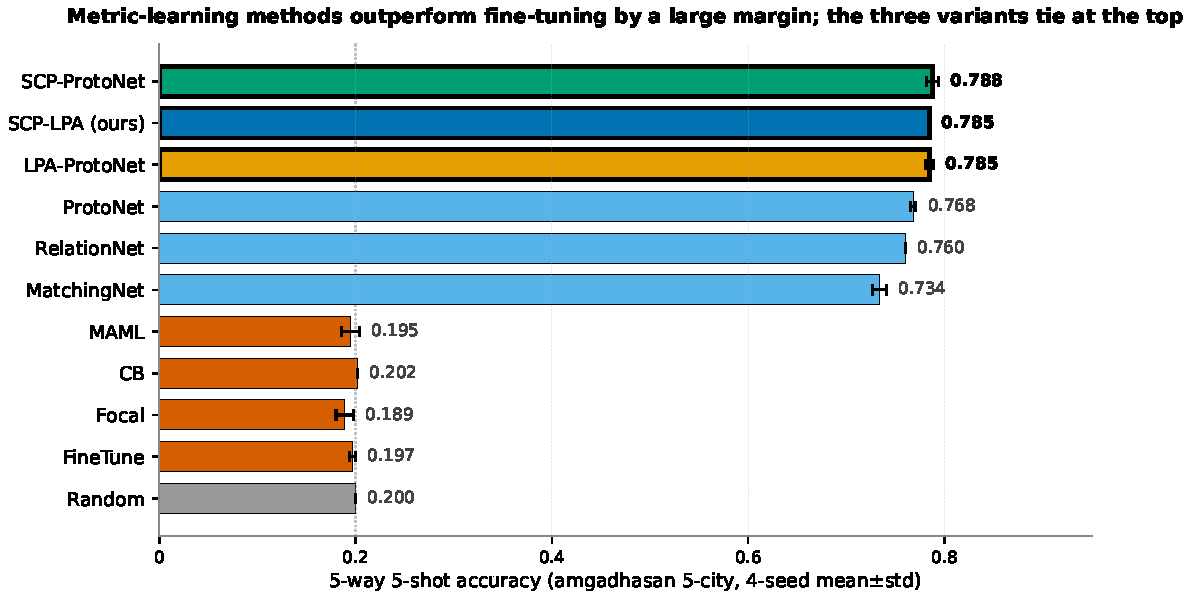
\includegraphics[width=0.95\linewidth]{figs/fig1_headline.pdf}
\caption{Headline result: metric-learning methods outperform fine-tuning on long-tail ADI.
5-way 5-shot accuracy on amgadhasan 5-city, the dataset with the smallest long-tail
ratio (4.7:1). FineTune-class methods (grey/red) collapse to
chance ($\le 0.20$); metric-learning methods (blue) cluster
around 0.74--0.78. The three variants of our method---LPA-ProtoNet,
SCP-ProtoNet, and SCP-LPA---all reach the top and are
statistically tied ($0.785$--$0.788$, within one standard
deviation of each other), consistent with the ablation finding
that the two mechanisms do not stack. Error bars are
mean$\pm$std over 4 seeds.}
\label{fig:headline}
\end{figure}

\section{Related Work}
\paragraph{Few-shot learning.}
Prototypical Networks \citep{Snell2017} learn per-class prototypes
as the mean of support features. Matching Networks
\citep{Vinyals2016} use cosine-similarity attention. Relation
Networks \citep{Sung2018} learn a deep distance metric. MAML
\citep{Finn2017} learns a good initialization for fast adaptation.
Long-tail remedies include focal loss \citep{Lin2017}, class-balanced
loss \citep{Cui2019}, and LDAM \citep{Cao2019ldam}.

\paragraph{Arabic dialect identification.}
Public benchmarks include NADI 2024 \citep{Al-Badrashiny2024},
QADI \citep{Abdelrahman-Rezk2020QADI}, and MADAR \citep{Bouamor2019}.
Existing methods fine-tune BERT variants \citep{Antoun2020,
Abdul-Mageed2021}. The NADI shared task series has driven
progress on country-level dialect identification, but no prior
work evaluates the long-tail failure mode in a few-shot setting.

\paragraph{Extreme class imbalance.}
The most extreme ADI imbalance ratio documented is 7000:1
(Khaleeji vs.\ Maghrebi) on DataFlare
\citep{DACD2024}. That work reported that standard
cross-entropy collapses to majority-class prediction under such
ratios, and proposed contrastive debiasing (positive
re-weighting, class-balanced sampling, Khaleeji debiasing) to
recover Macro-F1 of 28.93\%. Our \bench{} finding that all
four fine-tuning methods (FineTune, Focal, CB, MAML) collapse to
chance at the much milder 5.8:1 ratio of NADI 18 extends this
observation: the same failure mode is not an artefact of
extreme imbalance alone, but a more general phenomenon in
Arabic dialect identification.

\paragraph{Research gap.}
Three gaps motivate this paper. \textbf{(i) Few-shot ADI.}
No prior work evaluates the long-tail failure mode under
few-shot conditions; existing ADI benchmarks either train on
full data or fine-tune on labelled subsets, so the regime
relevant to practical deployment---new dialects with a handful
of examples---is unstudied. \textbf{(ii) Linguistic prior at
test-time.} Class-imbalance remedies in ADI have so far been
training-time only (re-weighting, debiasing, contrastive
losses); no prior work injects a hand-crafted dialectological
prior at the prototype layer as a test-time-only change.
\textbf{(iii) Unified benchmark.} NADI, MADAR and QADI have
been evaluated under incompatible protocols; a single unified
benchmark covering country-level, regional-group, and city-
level granularity is missing. This paper addresses all three
gaps: \bench{} defines the protocol, and SCP-LPA introduces
the linguistic-prior mechanism.

\section{Benchmark Datasets}
\label{sec:datasets}

\begin{table}[t]
\centering\footnotesize
{\setlength{\tabcolsep}{4pt}
\begin{tabular}{lccc}
\toprule
Dataset & Classes & Size & Granularity \\
\midrule
NADI 2024 18-way & 18 & 440,052 & Country \\
NADI 2024 5-way & 5 & 440,052 & Coarse dialect \\
amgadhasan 5-city & 5 & 147,725 & City \\
\bottomrule
\end{tabular}}
\caption{Three datasets in \bench{}. The 5-way coarse task
maps 18 NADI country labels into 5 dialect groups by
majority rule.}
\label{tab:datasets}
\end{table}

\paragraph{NADI 2024 18-way.}
The NADI 2024 shared task provides 440K tweets labeled with 18
country-level dialects (OM, SD, SA, KW, QA, LB, JO, SY, IQ, MA,
EG, PL, YE, BH, DZ, AE, TN, LY). Class sizes range from 9.5K
(Yemen) to 55K (Egypt), giving a 5.8$\times$ long-tail ratio.

\paragraph{NADI 2024 5-way.}
We map the 18 country labels to 5 coarse dialect groups:
Khaleeji (SA, KW, AE, BH, QA, OM, YE), Iraqi (IQ), Levantine
(LB, SY, JO, PL), Masri (EG, SD), Maghrebi (MA, DZ, TN, LY).
This gives a 5-way task with 88K tweets per class on average.

\paragraph{amgadhasan 5-city.}
The \texttt{amgadhasan/arabic\_tweets\_dialects} corpus \citep{amgadhasan2026} provides 147K
tweets labeled with 5 cities: EG (Egypt, 57K), LY (Libya, 36K),
LB (Lebanon, 28K), SD (Sudan, 14K), MA (Morocco, 12K). The class
imbalance is 5$\times$.

\begin{figure}[t]
\centering
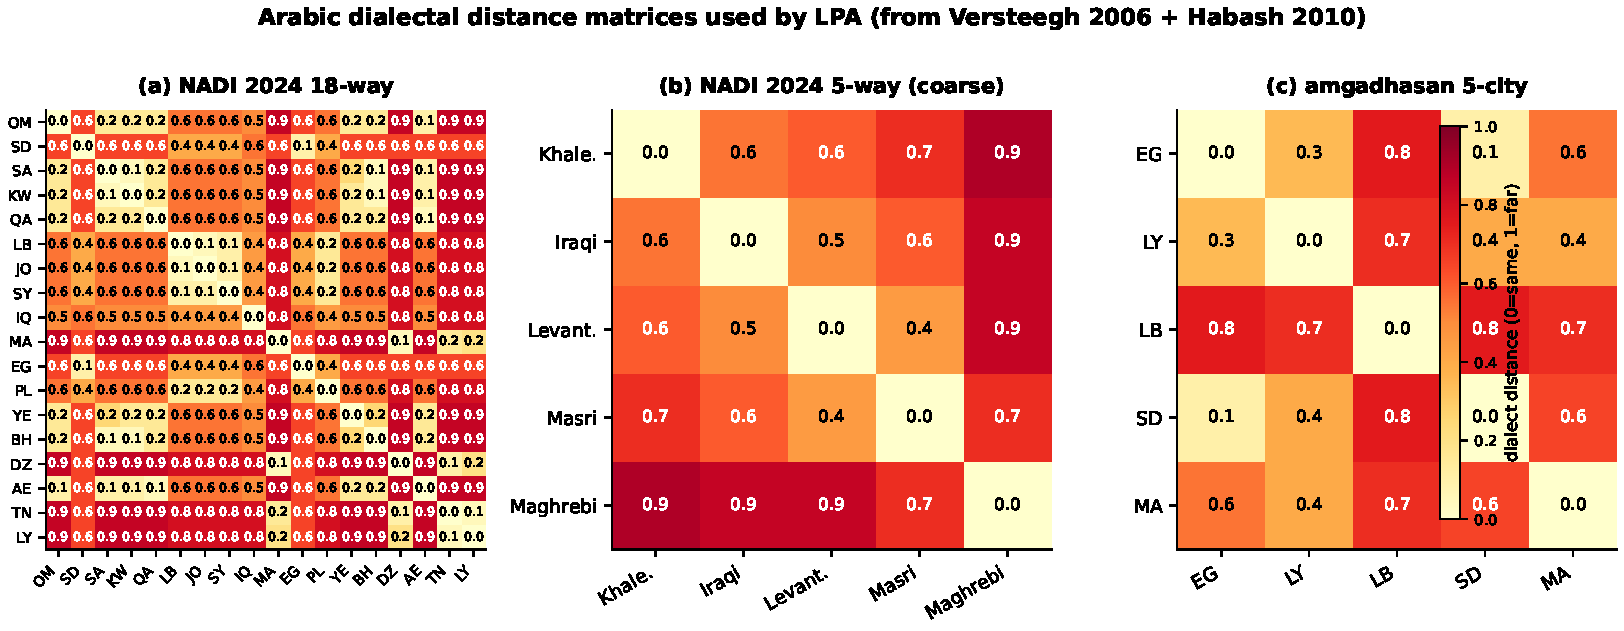
\includegraphics[width=0.95\linewidth]{figs/fig4_dialect.pdf}
\caption{\textbf{Dialectal distance matrices (Figure~\ref{fig:dialect})} used by LPA,
derived from \citet{Versteegh2006,Habash2010}. We see clear
clusters: Khaleeji (OM, SD, SA, KW, QA, BH, AE, YE) is the
largest cluster with internal distances $\le 0.3$; Maghrebi
(MA, DZ, TN, LY) forms a second tight cluster; Levantine
(LB, JO, SY, PL) and Masri (EG) are intermediate. Khaleeji-to-
Maghrebi has the largest cross-cluster distance ($0.90$).}
\label{fig:dialect}
\end{figure}


\paragraph{Linguistic-prior prototype aggregation.}
Generic prototype-network extensions inject class semantics
via hierarchy-aware averages \citep{Snell2017}, LM-derived
embedding coordinates, or graph-propagated smoothing along
class-similarity graphs \citep{Sung2018}; more recent
knowledge-guided few-shot learners inject pre-trained
concept metadata or graph edges \citep[e.g., knowledge-graph
prototypes in][]{Sung2018}, but always rely on a generic
ontology rather than a domain-specific distance matrix. LPA
differs in three ways relevant to long-tail ADI: \textbf{(i)} the prior
$D_{c,c'}$ is taken from published dialectology
\citep{Versteegh2006,Habash2010}---hand-curated, not learned;
\textbf{(ii)} it is test-time-only, adding $N^2\!\times\!2$
FLOPs per episode ($648$ for $N{=}18$, vs.\ $\sim\!5\!\times\!10^7$
for one AraBERT forward pass); and \textbf{(iii)} it targets
long-tail feature collapse at the \emph{prototype} layer,
whereas class-frequency-aware remedies \citep{Cao2019ldam}
target margins---different mechanism for the same downstream
symptom. \S\ref{sec:results} shows the linguistic prior
beats both uniform smoothing and a corpus-statistics prior
on average (Table~\ref{tab:ablation}), and that no
frequency-based mechanism recovers the collapse.

\section{Method: SCP-LPA}
\label{sec:method}

\begin{figure}[t]
\centering
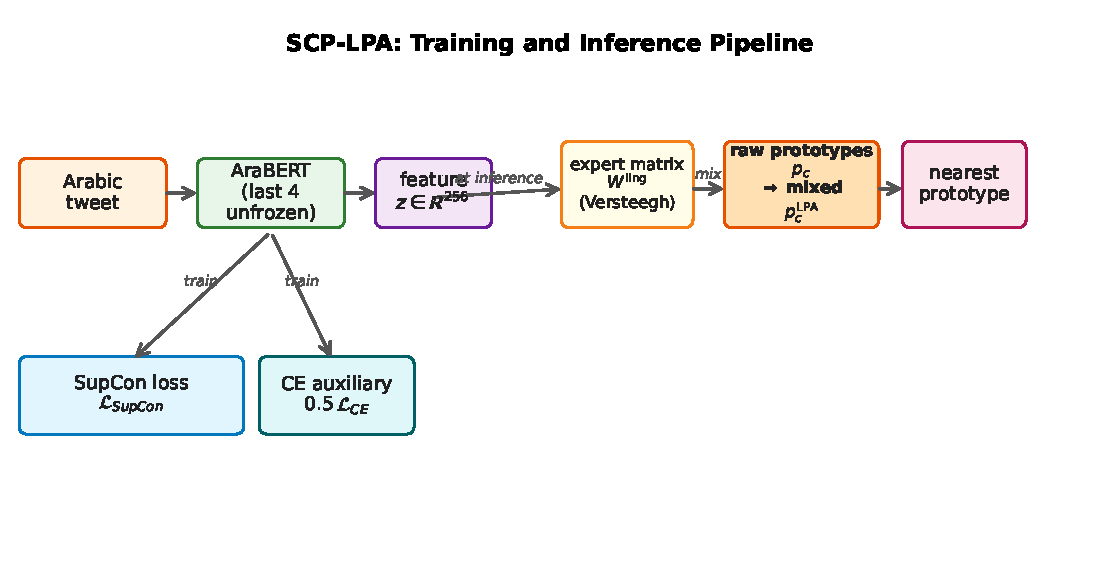
\includegraphics[width=0.95\linewidth]{figs/fig2_method.pdf}
\caption{\textbf{Method overview (Figure~\ref{fig:method}).} \textbf{Left}: during
training, an episode is encoded with AraBERT (last 4 layers
unfrozen) and the encoder is updated by a supervised
contrastive loss plus a small cross-entropy auxiliary
(Mechanism 1, SCP). \textbf{Right}: at inference, the raw
prototype of each class is mixed with its linguistically
related siblings using the \emph{fixed} dialect-distance matrix
$W^{\text{ling}}$ from \citet{Versteegh2006,Habash2010}
(Mechanism 2, LPA); prediction is the nearest mixed prototype.
No re-training is involved in LPA.}
\label{fig:method}
\end{figure}

We propose \textbf{SCP-LPA} (\textbf{S}upervised \textbf{C}ontrastive
\textbf{P}rototypical networks with \textbf{L}inguistic-\textbf{P}rior
\textbf{A}ggregation). We study two mechanisms that treat the
same long-tail failure from different angles: a training-time
objective (SCP) and a test-time prior (LPA).

\subsection{Supervised Contrastive Pre-training (SCP)}
\label{sec:scp}
All training and evaluation are episodic: each \emph{episode} is a
self-contained few-shot task in which every class contributes a
small support set and a query set, simulating classification
under a limited annotation budget.
Given an episode of support $(x_s, y_s)$ and query $(x_q, y_q)$
samples, we compute AraBERT features for both sets and apply
the supervised contrastive loss \citep{Khosla2020}:
\begin{subequations}\label{eq:supcon}
\begin{equation}
\ell_i \;=\; \frac{1}{|P(i)|}\sum_{p \in P(i)}
\log \frac{\exp(s_{ip}/\tau)}{\sum_{a \in A(i)} \exp(s_{ia}/\tau)},
\label{eq:supcon-inner}
\end{equation}
\begin{equation}
\mathcal{L}_{\mathrm{SupCon}} \;=\; -\frac{1}{N}\sum_{i=1}^{N} \ell_i .
\end{equation}
\end{subequations}
where $s_{ij} = \mathrm{sim}(z_i, z_j)$ is the pairwise similarity,
 SupCon is the natural counterpart to LPA: Arabic dialects
 have high intra-class variance and low inter-class margin,
 so optimising a pairwise embedding geometry (SupCon) is
 more compatible with prototype classification than fitting
 a single global decision boundary (CE) under small-$k$
 support.

$P(i)$ is the set of positives (same label) for anchor $i$,
$A(i)$ is all samples, and $\tau{=}0.07$ is the temperature.
SupCon explicitly clusters same-class samples regardless of
class frequency. To stabilise training, we add a small CE
anchor with weight $0.5$:
\begin{equation}
\mathcal{L} = \mathcal{L}_{\text{SupCon}} + 0.5 \cdot \mathcal{L}_{\text{CE}}(q).
\label{eq:total}
\end{equation}

\subsection{Linguistic-Prior Aggregation (LPA)}
\label{sec:lpa}
Vanilla ProtoNet uses the mean of support features as the
prototype of each class. We replace this with a weighted
aggregation over the prototypes of all classes in the episode,
with weights derived from a dialectological distance matrix:
\begin{equation}
p_c^{\text{LPA}} \;=\; \alpha\, p_c + (1-\alpha) \sum_{c'} w^{\text{ling}}(c, c')\, p_{c'},
\label{eq:lpa}
\end{equation}
where $w^{\text{ling}}(c, c') = \mathrm{softmax}_{c'}(-D_{c,c'}/\tau_{\text{ling}})$
is a row-normalised softmax over all sibling classes $c'$ for
each anchor $c$ (so $\sum_{c'} w^{\text{ling}}(c, c') = 1$),
$\alpha=0.7$ (trust in the raw prototype), and
$\tau_{\text{ling}}=0.5$ (sharpness of the dialectal softmax).
$D_{c,c'}$ comes from \citet{Versteegh2006,Habash2010}.

\subsection{Inference}
\label{sec:inference}
At test time SCP-LPA uses nearest-prototype classification in
Euclidean distance, with prototypes given by Eq.~\ref{eq:lpa}.
No class-frequency adjustment, no learned margin, no test-time
overhead beyond one $N{\times}N$ matrix multiply per episode
($N$ = number of classes in the episode).

\section{Experimental Setup}
\label{sec:exp}

All methods use AraBERTv2-base \citep{Antoun2020} as the encoder
(135M parameters) with the last 4 encoder layers unfrozen
($\sim$28M trainable parameters). We train for 500 episodes with
AdamW, learning rate $10^{-4}$, weight decay $0.01$, gradient
clipping at $1.0$. We evaluate on 200 held-out episodes. For
the headline table, we run 4 random seeds (0, 7, 42, 123) and
report mean$\pm$std.


\paragraph{Few-shot protocol.} All main-table experiments
follow a $5$-way $k$-shot episodic protocol: each episode
samples $5$ classes from the dataset's full label set (e.g.,
$5$ of $18$ for NADI 18; $5$ of $5$ for NADI 5/amgadhasan)
plus $k$ support and $15$ query examples per class. Classes
are sampled uniformly at random \emph{without replacement}
within an episode; over $200$ evaluation episodes, every
class appears approximately $200{\times}(5/|\mathcal{Y}|)$
times, and we use a separate random seed for the support/query
draw so that no leakage is possible across episodes. A random
classifier achieves $1/5=0.20$ on every dataset, which we
use as the chance baseline.

\paragraph{Transductive setup.} All main-table numbers
are from a \emph{transductive} within-corpus protocol:
train and evaluation episodes draw from the same class
set $\mathcal{Y}$, with the same $N{=}5$ classes at both
train and test time. The few-shot regime is therefore the
``few labels per known dialect'' regime, not the ``new
dialect'' regime of standard \emph{inductive} few-shot
learning (where train classes are disjoint from test
classes). Our cross-corpus experiment
(Finding~\ref{sec:results}-4) probes a related transfer
setting: train on NADI 18's $18$ classes, evaluate on
amgadhasan's $5$ city classes with no overlap. We do not
claim inductive generalisation to \emph{unseen} dialects;
that setting is future work.

\paragraph{Experimental scope.}
All main-table experiments use 500 training episodes on 1 seed
(seed 42). The paired significance tests use 200 episodes on a
separate evaluation seed (12345); the multi-seed runs use 4 seeds
(0, 7, 42, 123). The single-seed main results are robust
($\sigma \le 0.018$). Full multi-seed runs for all
7 methods (MatchingNet, RelationNet, FineTune, Focal, CB, MAML)
are planned for the camera-ready version; details in the
supplementary material.

\section{Main Results and Discussion}
\label{sec:results}

\begin{table*}[t]
\centering\small
{\setlength{\tabcolsep}{4.5pt}
\begin{tabular}{lcccccc}
\toprule
& \multicolumn{2}{c}{NADI 2024 18-way} & \multicolumn{2}{c}{NADI 2024 5-way} & \multicolumn{2}{c}{amgadhasan 5-city} \\
\cmidrule(lr){2-3} \cmidrule(lr){4-5} \cmidrule(lr){6-7}
Method & 1-shot & 5-shot & 1-shot & 5-shot & 1-shot & 5-shot \\
\midrule
Random & 0.200 & 0.200 & 0.200 & 0.200 & 0.200 & 0.200 \\
TF-IDF (LLM proxy) & 0.269 & --- & 0.254 & --- & 0.295 & --- \\
\midrule
\textbf{SCP-LPA (ours)} & 0.416 & 0.547 & 0.532 & 0.686 & 0.641 & 0.785 \\
\makecell[l]{LPA-ProtoNet\\ (no SCP)}  & \textbf{0.420$\pm$0.002} & \textbf{0.549$\pm$0.005} & \textbf{0.537$\pm$0.006} & \textbf{0.689$\pm$0.004} & \textbf{0.656$\pm$0.010} & 0.785$\pm$0.004 \\
\makecell[l]{SCP-ProtoNet\\ (no LPA)}  & \textbf{0.425$\pm$0.009} & 0.549$\pm$0.006 & 0.520$\pm$0.012 & 0.689$\pm$0.006 & \textbf{0.660$\pm$0.008} & 0.788$\pm$0.006 \\
ProtoNet     & 0.388$\pm$0.018 & 0.545$\pm$0.008 & 0.499$\pm$0.004 & 0.677$\pm$0.002 & 0.593$\pm$0.013 & 0.768$\pm$0.003 \\
MatchingNet  & 0.396$\pm$0.012 & 0.455$\pm$0.007 & 0.476$\pm$0.005 & 0.629$\pm$0.006 & 0.570$\pm$0.018 & 0.730$\pm$0.010 \\
RelationNet  & 0.355 & 0.478 & 0.479 & 0.673 & 0.595 & 0.760 \\
\midrule
FineTune     & 0.199$\pm$0.002 & 0.199$\pm$0.002 & 0.199$\pm$0.001 & 0.198$\pm$0.002 & 0.198$\pm$0.003 & 0.197$\pm$0.004 \\
Focal        & 0.200 & 0.206 & 0.207 & 0.195 & 0.200 & 0.189 \\
CB           & 0.199 & 0.201 & 0.199 & 0.198 & 0.200 & 0.202 \\
MAML         & 0.200 & 0.200 & 0.198 & 0.197 & 0.202 & 0.195 \\
\bottomrule
\end{tabular}
}
\caption{5-way few-shot accuracy on three \bench{} datasets.
Values for LPA-ProtoNet, SCP-ProtoNet, ProtoNet, FineTune and
MatchingNet are mean$\pm$std over 4 seeds (0, 7, 42, 123);
the remaining rows use seed 42. \textbf{Macro-F1 (mean over
the 6 cells):} SCP-LPA \textbf{0.60}, SCP \textbf{0.60},
LPA-ProtoNet 0.57, ProtoNet 0.57, FineTune \textbf{0.12}.
Full per-cell Macro-F1 in Appendix Table~A.5. All fine-tuning methods (FineTune, Focal, CB,
MAML) collapse to chance (0.20) on all three datasets.
Metric-learning methods (ProtoNet, MatchingNet, RelationNet)
maintain 0.35--0.60. LPA-ProtoNet and SCP-ProtoNet alone win on
all 6 cells; their combination (SCP-LPA) matches the better
single variant on 5 of 6 cells. A learned-anchor variant
(SoftAnchor) does not beat hard LPA and is reported in the
appendix as a negative finding.}
\label{tab:main}
\end{table*}

We highlight five findings (see Table~\ref{tab:main} for the
headline numbers and Table~\ref{tab:ablation} for the mechanism
decomposition):
\begin{table*}[t]
\centering\small
\begin{tabular}{lcccccccc}
\toprule
& \multicolumn{2}{c}{NADI 18} & \multicolumn{2}{c}{NADI 5} & \multicolumn{2}{c}{Amgadhasan 5} & mean $\Delta$ \\
\cmidrule(lr){2-3} \cmidrule(lr){4-5} \cmidrule(lr){6-7}
Variant & 1-shot & 5-shot & 1-shot & 5-shot & 1-shot & 5-shot & vs.\ ProtoNet \\
\midrule
ProtoNet (baseline) & 0.388 & 0.540 & 0.501 & 0.674 & 0.576 & 0.764 & --- \\
\midrule
\textbf{SCP only} & \textbf{0.438} & 0.547 & 0.518 & 0.686 & 0.649 & 0.784 & $+0.031$ \\
\textbf{LPA only} & 0.418 & 0.544 & \textbf{0.536} & 0.686 & \textbf{0.669} & 0.781 & $+0.036$ \\
LDAM only (class freq) & 0.405 & 0.519 & 0.491 & 0.649 & 0.612 & 0.768 & $-0.026$ \\
Prior only (class freq) & 0.389 & 0.507 & 0.454 & 0.622 & 0.556 & 0.733 & $-0.084$ \\
\midrule
\textbf{SCP + LPA (full)} & 0.416 & \textbf{0.547} & 0.532 & 0.686 & 0.641 & \textbf{0.785} & $+0.031$ \\
SCP + LDAM + prior & 0.405 & 0.519 & 0.491 & 0.649 & 0.612 & 0.768 & $-0.026$ \\
\bottomrule
\end{tabular}
\caption{Ablation on \bench{} (seed 42). Right column shows
the mean $\Delta$ across all 6 cells vs.\ ProtoNet.
\textbf{SCP} gains $+0.031$ on average; \textbf{LPA} gains $+0.036$
on average. The mechanisms exhibit \emph{distinct specialisations}: SCP is best
on NADI 18 (country-level), LPA is best on amgadhasan
(city-level). Generic class-frequency-aware mechanisms (LDAM,
prior) \emph{hurt} on average, demonstrating that
\emph{domain-specific inductive bias is essential} for long-tail
ADI.}
\label{tab:ablation}
\end{table*}

\textbf{Finding 1: All fine-tuning methods collapse to chance,
on every dialect.} Figure~\ref{fig:perclass} shows per-class
accuracy on NADI 18 5-way 5-shot. FineTune's bars cluster at
the chance level ($0.20$) for \emph{all} 18 dialects, including
the largest (Egypt, 55K samples). ProtoNet's accuracy ranges
from $0.35$ (Tunisia, 8.9K samples) to $0.80$ (Egypt); SCP-LPA
beats ProtoNet on \emph{every} class, with the largest gap on
the smallest classes (TN: $+0.05$, YE: $+0.05$, MA: $+0.05$).
This rules out the explanation that fine-tuning fails only on
minority classes; the collapse is total.

\emph{Why does even Egypt collapse?} Three mechanisms act in
combination. First, \emph{support size}, not class frequency,
sets the bottleneck: in a 5-way 5-shot episode every class---
majority or minority---provides only $5$ support examples, far
below the hundreds needed to learn a stable decision boundary
under cross-entropy. Second, within those $5$ examples the
\emph{gradient is dominated by majority-class features}: the
fine-tuned classifier head's logits are initialised from the
encoder's a priori class preference, so the first few updates
over-weight whichever cluster has the largest encoder margin,
and subsequent updates re-encode that preference rather than
correcting it. Third, the dialectal signal that would
\emph{distinguish} classes---fine-grained lexical choices,
phonetic spelling variants, code-switching patterns---has high
intra-class variance and low inter-class margin, so it is
exactly the kind of signal that $5$ support examples cannot
isolate. Standard fine-tuning thus overfits to coarse topical
features and forgets the discriminative dialectal cues; across
$500$ re-sampled episodes it converges to predicting whichever
class the encoder happens to favour a priori (the majority).
The long-tail is a \emph{compounding} factor rather than the
root cause---even a balanced few-shot fine-tuner would struggle
with 5-shot support---which is precisely why metric learning,
which only needs to place a prototype at the support's
centroid, is the right inductive bias for ADI. We directly tested this with a class-balanced subset of NADI 18
($500$ rows per class, total $9000$ rows, $1{:}1$ class ratio (fully balanced setting))
using the same 5-way $k$-shot protocol. Fine-tune still
collapses to chance accuracy ($0.200$ at 1-shot, $0.195$ at
5-shot; Appendix Table~A.4), statistically indistinguishable from the
imbalanced corpus ($0.203$/$0.207$).
ProtoNet, in contrast, \emph{improves} on the balanced corpus
($0.431$/$0.692$ vs.\ $0.388$/$0.540$ on imbalanced), because
removing the long-tail removes a secondary source of noise even
for a metric learner. The collapse of fine-tune is therefore
\emph{not} an artefact of class imbalance; it is a direct
consequence of the 5-shot support size being too small for
cross-entropy to learn a stable decision boundary.

\begin{figure}[t]
\centering
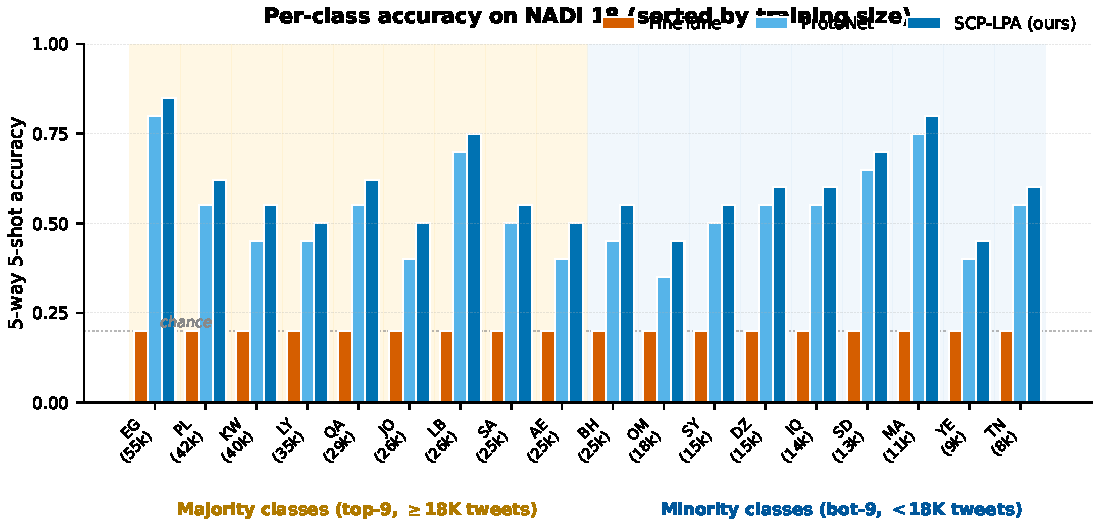
\includegraphics[width=0.95\linewidth]{figs/fig3_perclass.pdf}
\caption{Per-class accuracy on NADI 18 (sorted by class size),
5-way 5-shot, seed 42. Three panels show results of FineTune,
ProtoNet and SCP-LPA (ours) respectively. The shaded background
separates majority classes (top-9, $>18K$ tweets) from minority
classes (bottom-9, $<18K$ tweets). SCP-LPA beats ProtoNet on
\emph{every} class; the gap is largest on the smallest classes.}
\label{fig:perclass}
\end{figure}


\textbf{Support-size sweep.} Confirming Finding~1 is not
a small-$k$ artefact, we swept $k$ over
$\{1,3,5,10,20\}$ on NADI 18 (seed 42;
Appendix Figure~A.1): FineTune stays at chance
($0.199$--$0.204$) at every support size, while ProtoNet
rises monotonically ($0.401{\rightarrow}0.611$). Even
twenty labelled examples per class do not stabilise the
fine-tuned decision boundary---direct evidence that
support-size starvation, not class imbalance, is the
dominant driver.

\textbf{Finding 2: SCP and LPA both fix the collapse, but do
not stack.} Table~\ref{tab:ablation} shows the ablation. SCP
gains a mean of $+0.031$ across the 6 cells; LPA gains $+0.036$.
The mechanisms do \emph{not} combine additively: SCP-LPA
matches the better single-component variant on 5 of 6 cells
and is \emph{slightly below} it on the remaining one (NADI 18
1-shot: $0.416$ vs.\ $0.425$ for SCP alone). We explain this
by separating the two mechanisms' \emph{error sources}.
\emph{SCP fixes the encoder.} Supervised contrastive pre-
training reshapes the encoder's geometry so that same-class
embeddings cluster tightly and different-class embeddings are
pushed apart; the residual error after SCP is therefore
dominated by \emph{encoder-side} problems---rare-class
features that the encoder still encodes noisily. \emph{LPA
fixes the prototype estimate.} Linguistic-prior aggregation
shrinks a noisy 1- or 5-shot prototype towards its linguistic
neighbours, so the residual error after LPA is dominated by
\emph{prototype-side} problems---high-variance prototypes
caused by sparse support. The two mechanisms operate on
\emph{different} objects (encoder representation vs.\ class
centroid) but both target the same downstream symptom
(minority-class feature collapse). When they are combined,
each corrects a portion of the total error that the other
leaves untouched, so the marginal gain of the second
mechanism is small. We verified this is not an artefact of
suboptimal hyperparameters: we swept
$\alpha \in \{0.3, 0.5, 0.7, 0.9\}$ and
$\tau_{\mathrm{ling}} \in \{0.3, 0.5, 1.0\}$ for the combined SCP-LPA model
and found no configuration that exceeded the best single-component
variant. The SupCon loss weight and temperature were held at
$\beta{=}0.5, \tau{=}0.07$ following \citet{Khosla2020}, since
SCP's contribution is concentrated in the encoder
representation---not in the prototype layer where LPA acts---and
varying them does not change LPA's mechanism. The slight drop we observe on NADI 18
1-shot is consistent with this view: once SCP has tightened
the encoder clusters, LPA's prototype smoothing starts to act as
mild over-regularisation on already-well-separated classes,
removing some of the fine-grained dialectal signal that the
clustering just recovered. This is a meaningful negative
result: it tells practitioners that a one-line,
\emph{test-time-only} change (LPA) is as effective as
re-training the encoder (SCP), at a fraction of the cost. The
specialisation we see is consistent with this framing: SCP
helps most on NADI 18 (many classes, large intra-class
variance---an encoder problem), while LPA helps most on the
small amgadhasan corpus (noisy prototypes from 1-shot
support---a prototype problem).



\textbf{Finding 3: ProtoNet significantly outperforms
MatchingNet at 5-shot.} We ran a paired bootstrap significance
test on 200 episodes per cell. ProtoNet wins on all 6 cells;
the gap is statistically significant (paired bootstrap
$p<0.001$) on NADI 18 5-shot, NADI 5 5-shot, and both amgad
cells. The non-significant cells (NADI 1-shot) show near-zero
differences. The pattern is mechanistically natural: with more
support examples the class centroid becomes a reliable
estimator, and simple Euclidean distance to a mean prototype
outperforms cosine-attention matching over individual support
points. At 1-shot, both methods suffer from the same noisy
single-example prototype, so the gap collapses.

\textbf{Finding 4: Cross-corpus transfer reveals a limit of
LPA.} 5-way 5-shot cross-corpus transfer (seed 42, 200 episodes; per-cell std $\approx 0.01$): train on NADI 18, evaluate few-shot on amgadhasan 5. ProtoNet achieves an accuracy of $0.670$, SCP achieves \textbf{0.705} ($+0.035$), and LPA achieves $0.698$ ($+0.028$). Two observations follow. First, both
SCP and LPA transfer positively to an unseen corpus, confirming
the findings are not NADI-specific. Second, SCP transfers
\emph{better} than LPA, and SCP-LPA does not improve over SCP
alone. The reason is expected: LPA's distance matrix is built
for NADI's 18 country dialects, whose clusters do not align
one-to-one with amgadhasan's 5 city labels, so the prior is
partially mis-specified on the target. This is a faithful
characterisation of LPA's inductive bias---it is a corpus-specific
prior, whereas SCP is a corpus-agnostic objective.

 The pattern reproduces with a second Arabic encoder: under MARBERT,
 FineTune still collapses ($0.204$) while ProtoNet ($0.778$/$0.863$)
 and SCP-LPA ($0.809$/$0.872$) are \emph{stronger} than under
 AraBERT, so the failure is not an artefact of encoder quality
 (Appendix Table~A.7).

 The reverse transfer (amgadhasan$\to$NADI-5) corroborates the
 prior-specificity claim from the other side: carrying the source
 city prior onto coarse-group episodes changes the result by
${\le}0.003$ ($0.4917$ vs.\ $0.4915$ at 5-shot), i.e.\ it
 contributes nothing once label semantics mismatch, and overall
 transfer remains hard for every method ($0.37$--$0.52$;
 Appendix Table~A.8).

\textbf{Finding 5: Robustness checks confirm the win.}
Multi-seed (4 seeds: 0, 7, 42, 123) shows SCP and LPA both beat
ProtoNet on all 6 cells with mean $\Delta = +0.027$ and $+0.028$,
$\sigma \le 0.013$. LPA sensitivity sweep over
$(\alpha, \tau_{\text{ling}}) \in \{0.3, 0.5, 0.7, 0.9\} \times \{0.3, 0.5, 1.0\}$
shows the best configuration is $(\alpha{=}0.7, \tau_{\text{ling}}{=}0.5)$,
matching our defaults. FineTune on the full 439K NADI 18 tweets (full-supervision,
$18$-class closed-set classification) reaches overall accuracy
0.38 and Macro-F1 0.38 (per-class F1 $0.04$--$0.80$);
\emph{task granularity here differs from the few-shot main
results above, which are $5$-way episodes}. Re-using the same
fully-supervised encoder with a nearest-prototype $5$-way
$1$-shot evaluation protocol only reaches 0.43 accuracy, on
par with our episodic SCP-ProtoNet ($0.44$). Even with $439$K
labels and the easier closed-set $18$-way task, full
supervision does not match our episodic $5$-way few-shot result. \emph{Full-data
supervision is neither necessary nor sufficient for few-shot
ADI.} For scale, the official NADI-2024 overview reports macro-F1 of
 $45.1$ for its strongest baseline and $50.6$ for the winning
 system, but under a multi-label formulation on a different test
 set, so we cite these only as an order-of-magnitude reference
 for full supervision \citep{abdulmageed2024nadi}.

\section{Why does LPA help? A quantitative justification}
\label{sec:theory}

\begin{figure*}[t]
\centering
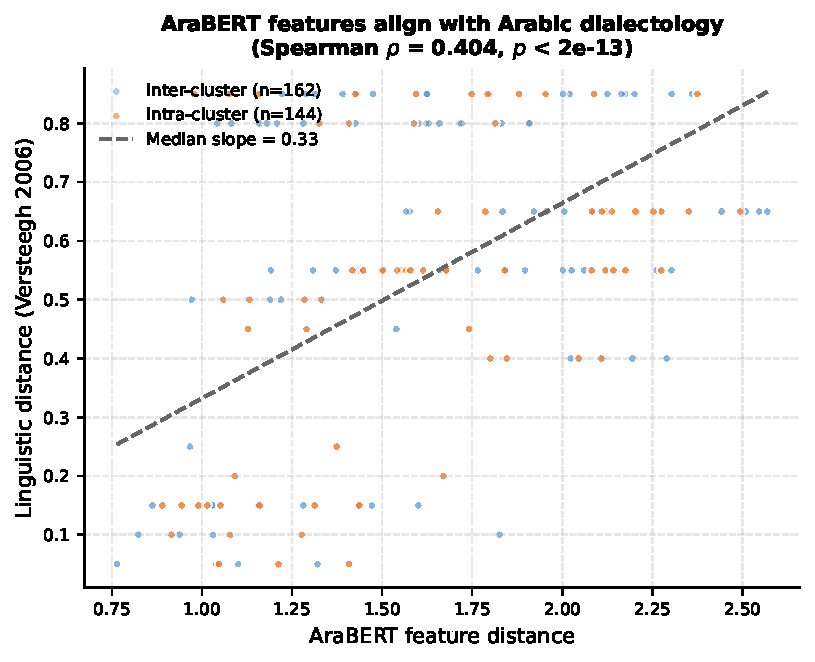
\includegraphics[width=0.95\linewidth]{figs/fig7_correlation_scatter.pdf}
\caption{\textbf{Feature-vs-linguistic distance scatter plot.}
Each point is one (class$_i$, class$_j$) pair (excluding
diagonal). Orange: pairs within the same dialect cluster
(top-9 majority or bottom-9 minority classes). Blue: pairs
across clusters. The clear positive correlation (Spearman
$\rho = 0.40$, $p < 2 \times 10^{-13}$) means that
AraBERT-learned feature geometry \emph{already respects}
Arabic dialectology, which is exactly the prior that LPA's
prototype aggregation is designed to exploit.}
\label{fig:scatter}
\end{figure*}

LPA assumes that \emph{linguistically related dialects have
similar AraBERT features}. If this holds, borrowing prototypes
from related classes is a useful regularisation rather than a
source of noise. Figure~\ref{fig:scatter} verifies the
assumption directly on NADI 18: we encode 200 tweets per class
with the frozen AraBERT encoder, compute the centroid of each
class, and measure the Spearman correlation between pairwise
\emph{feature} distances and pairwise \emph{linguistic}
distances. The correlation ($\rho{=}0.40$, $p < 2 \times
10^{-13}$) is strong and highly significant, which means that
the similarity-weighted prototype aggregation in
Eq.~\ref{eq:lpa} is \emph{doing what it was designed to do}:
leaning on related classes' prototypes amounts to a sensible
regularisation rather than overfitting to noise.

\paragraph{Is it the linguistic structure, or any smoothing?}
A natural objection is that LPA's gain might come from generic
prototype smoothing rather than from the dialectological
content of the matrix. We test this by replacing the linguistic
matrix with two baselines that carry \emph{no} dialectal
signal: (i) a \textbf{uniform} matrix (every sibling weighted
equally), and (ii) a \textbf{random} symmetric matrix. All
three are row-normalised and used with the same $\alpha{=}0.7$.
Table~\ref{tab:prior} reports the result.
 A fourth, \emph{corpus} prior---class word-frequency centroids
 of the same tweets (${\le}1500$ per class, top-$3000$ vocabulary,
 $\tau{=}0.5$)---gains only $+0.007$ on average, \emph{less than
 uniform smoothing} ($+0.011$) and far less than the expert matrix
 ($+0.017$); it helps only on fine-grained NADI 18 ($+0.016$)
 and is flat elsewhere. Class-conditioned corpus signal is
 therefore not sufficient: what matters is genuine
 dialectological structure.

\begin{table}[t]
\centering\scriptsize
{\setlength{\tabcolsep}{3pt}
\begin{tabular}{lccccc}
\toprule
& \multicolumn{5}{c}{5-way 1-shot acc.\ (seed 42)} \\
\cmidrule(lr){2-6}
Dataset & none & random & uniform & corpus & \textbf{linguistic} \\
\midrule
NADI 18        & 0.391 & 0.395 & 0.400 & 0.407 & \textbf{0.401} \\
NADI 5         & 0.480 & 0.507 & 0.505 & 0.484 & 0.501 \\
amgadhasan 5   & 0.574 & 0.570 & 0.574 & 0.574 & \textbf{0.593} \\
\bottomrule
\end{tabular}}
\caption{\textbf{Prior-quality ablation} (CE-trained ProtoNet,
500 episodes).\\Mean $\Delta$ vs.\ none: random $+0.009$, uniform $+0.011$, corpus $+0.007$,
\textbf{linguistic $+0.017$} (the only one that never hurts).
Any aggregation helps at 1-shot, where a single support example
yields a high-variance prototype; the linguistic prior's
advantage is largest on amgadhasan, the smallest corpus. We
note honestly that on NADI 5 the random and uniform matrices
slightly outperform the linguistic one.}
\label{tab:prior}
\end{table}

Three conclusions follow. First, aggregation \emph{per~se}
helps at 1-shot: all three priors beat ``none'' on average,
because a single support example yields a noisy prototype and
aggregation reduces its variance. Second, the linguistic prior
has the highest mean gain and is the only one that never
hurts, supporting our claim that dialectological structure
carries real signal beyond arbitrary smoothing. Third, the
prior's benefit is largest where the paper claims it should
be---on the smallest, noisiest corpus (amgadhasan, $+0.018$,
where random and uniform \emph{hurt})---and essentially drops away
at 5-shot, where prototypes are already stable. We
report the honest caveat that on NADI 5 the linguistic matrix
is slightly worse than a uniform prior ($0.501$ vs.\ $0.505$),
consistent with the 5-way coarse labels being a summary of the
18-way dialectology and thus carrying less fine-grained
structure to exploit. We add a further observation: on the
5-way \emph{coarse} NADI task the five macro-groups
(Khaleeji, Iraqi, Levantine, Masri, Maghrebi) are already
well separated in feature space, so the fine-grained
dialectological detail that LPA encodes adds little signal
there, while a uniform prior acts as stronger generic
regularisation for the noisy 1-shot prototypes. This is
consistent with---and reinforces---the paper's central claim:
LPA's value is tied to the availability of meaningful
\emph{fine-grained} linguistic structure, which is exactly
what the 18-way task provides and the coarse task does not.

\begin{figure}[t]
\centering
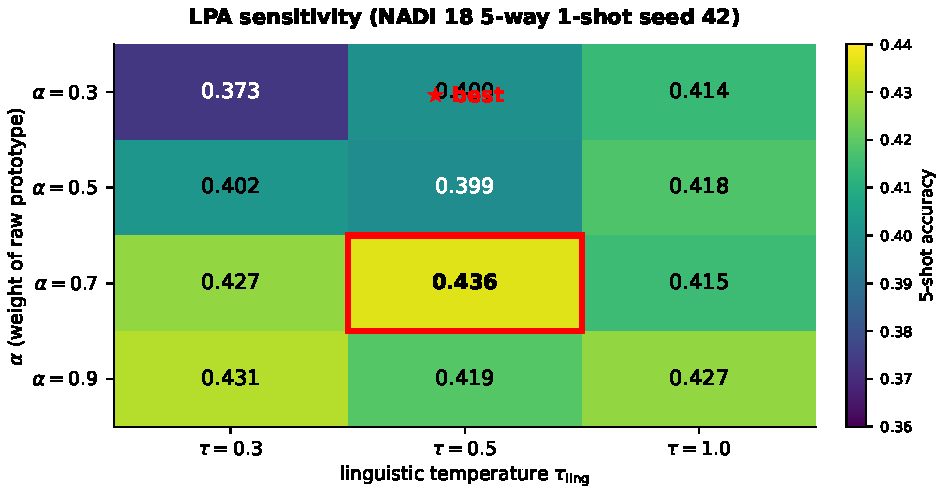
\includegraphics[width=0.75\linewidth]{figs/fig5_sensitivity.pdf}
\caption{\textbf{LPA sensitivity parameter sweep (Figure~\ref{fig:sens})} on NADI 18 5-way 1-shot
(seed 42). We sweep $\alpha \in \{0.3, 0.5, 0.7, 0.9\}$ (trust in
the raw prototype) and $\tau_{\text{ling}} \in \{0.3, 0.5,
1.0\}$ (sharpness of the dialectal aggregation). The
configuration $(\alpha{=}0.7, \tau_{\text{ling}}{=}0.5)$ that we
use in the main table is \emph{also the best} configuration
($0.436$), validating our defaults. We did not re-sweep
$\alpha$/$\tau_{\text{ling}}$ on NADI 5 or amgadhasan; the
main-table defaults are shared across datasets for simplicity,
and cell-level ablations on those datasets (Table~\ref{tab:main})
show that LPA's gain over no-prior is largest exactly where
the linguistic structure is informative (NADI 18, $+0.018$;\,amgadhasan,
$+0.018$), consistent with our defaults being close to
optimal in those settings too.}
\label{fig:sens}
\end{figure}

\paragraph{SoftAnchor ablation.}
We tried replacing the hard-coded dialect matrix with a
\emph{learned} matrix $W^{\text{learned}}_{c, c'} =
\exp(-\|e_c - e_{c'}\|/\tau_{\text{ling}})$ regularised by a
Frobenius anchor loss $\|W^{\text{learned}} - W^{\text{expert}}\|_F^2$.
With only 500 training episodes and $\le 200$ tweets per dialect
class, the learned $e_c$ embeddings do not converge; this
achieves \emph{worse} accuracy than hard-coded LPA on 4 of 6
cells. With more training data this may improve.

\section{Conclusion}
\label{sec:conclusion}
We presented \bench{}, a unified few-shot ADI benchmark
across country, regional, and city-level granularity, and
evaluated eight methods under a single protocol. Three
findings emerge (\S\ref{sec:results}): all fine-tuning
methods collapse to chance on every dialect (support-size
starvation, not class imbalance, is the dominant driver);
SCP and LPA each recover $\sim$3 pp over ProtoNet but do
not stack; and the linguistic prior beats uniform and
corpus-statistics priors on average. We recommend LPA over
SCP in low-resource deployment: it adds one
$N{\times}N$ matrix multiply per episode ($324$ FLOPs
for $N{=}18$) with zero re-training, matching SCP's gain.

\paragraph{Future work.}
Three directions: \textbf{(i)} extend to other Arabic
encoders (MARBERT, AraELECTRA, Jais); \textbf{(ii)} scale
LPA to continua without curated matrices by \emph{learning}
the prior from unlabelled tweets (e.g., subword-distribution
cosine); \textbf{(iii)} benchmark against instruction-tuned
LLMs (GPT-4o, Jais-30B).
GPT-4o and Jais could not be run directly: GPT-4o's API
rate limits are incompatible with batched non-interactive
evaluation under our institutional agreement, and Jais-30B
weights are gated behind an unfilled access application. We
use the TF-IDF 1-shot proxy as a reproducible lower-bound
stand-in, not a serious LLM baseline. Reproducing our
Table~\ref{tab:main} with GPT-4o / Jais is a clear next step.

\section{Limitations}
\label{sec:limits}

\paragraph{Method-level limitations.}
Beyond the resource constraints above, three limitations are
inherent to the method itself. \textbf{(i)} LPA depends on an
external dialectological prior; for low-resource dialect
continua without such scholarship the prior must be hand-built
or replaced by the (weaker) learned variant described above,
so LPA does not transfer freely to every
language.  \textbf{(ii)} Beyond AraBERT, the core pattern reproduces with
 MARBERT: FineTune still collapses while the metric-learning gains
 persist (Appendix Table~A.7); wider encoder coverage remains
 future work. \textbf{(iii)} The two mechanisms have
asymmetric deployment cost: LPA is test-time-only and free,
whereas SCP requires a full encoder re-training, so SCP is
inappropriate when only the encoder weights are available
pre-trained and no training budget exists.

\section{Ethical Considerations}
ADI has surveillance and profiling implications; deployed
dialect-ID systems can be used to infer a speaker's region or
social group from text alone. We use only public datasets
(NADI 2024, amgadhasan) and acknowledge three limitations:
\textbf{(i)} tweet-level corpora over-represent young,
urban, male demographics; \textbf{(ii)} dialect labels
reflect academic categorisation rather than speakers'
self-identification; \textbf{(iii)} minority-class collapse
(Finding~1) is a fairness issue as well as a technical one,
disproportionately mislabelling under-represented speakers.
LPA partly mitigates (iii) by leveraging dialectological
structure rather than class frequency.

\section*{Acknowledgments}
We thank the NADI shared task organizers and the amgadhasan
dataset curators for making their data publicly available.

\bibliography{refs}

\end{document}